% ************************************************************************
% 
% Fuzzy-Logic Based Detection and Characterization of Junctions and Terminations 
% in Fluorescence Microscopy Images of Neurons
%
% ************************************************************************
\chpos{15mm}{8mm}
\chapter[Fuzzy-Logic Based Detection and Characterization of Junctions and Terminations in Fluorescence Microscopy Images of Neurons]{Fuzzy-Logic Based Detection and Characterization of Junctions and Terminations in Fluorescence Microscopy Images of Neurons}
\chaptermark{Fuzzy-Logic Based Detection of Junctions and Terminations}
\label{ch2:fuzzy}

% [lraise=0.1, nindent=0em, slope=-.5em]
\myabstract{\lettrine{D}{igital} reconstruction of neuronal cell morphology is an important step toward understanding the functionality of neuronal networks. Neurons are tree-like structures whose description depends critically on the junctions and terminations, collectively called critical points, making the correct localization and identification of these points a crucial task in the reconstruction process. Here we present a fully automatic method for the integrated detection and characterization of both types of critical points in fluorescence microscopy images of neurons. In view of the majority of our current studies, which are based on cultured neurons, we describe and evaluate the method for application to two-dimensional (2D) images. The method relies on directional filtering and angular profile analysis to extract essential features about the main streamlines at any location in an image, and employs fuzzy logic with carefully designed rules to reason about the feature values in order to make well-informed decisions about the presence of a critical point and its type. Experiments on simulated as well as real images of neurons demonstrate the detection performance of our method. A comparison with the output of two existing neuron reconstruction methods reveals that our method achieves substantially higher detection rates and could provide beneficial information to the reconstruction process.}
\vspace*{13.0em}
% ************************************************************************
\begin{publish}
Based upon: M. Radojevi\'{c}, I. Smal, E. Meijering, ``Fuzzy-Logic Based Detection and Characterization of Junctions and Terminations in Fluorescence Microscopy Images of Neurons'', \textit{Neuroinformatics}, vol. 11, no. 11, pp.1-11, 2015.   
\end{publish}

\section{Introduction}
\label{ch2_sec_intro}
The complexity and functionality of the brain depend critically on the morphology and related interconnectivity of its neuronal cells \cite{kandel2000principles, ascoli2002computational, donohue2008comparative}. To understand how a healthy brain processes information and how this capacity is negatively affected by psychiatric and neurodegenerative diseases \cite{anderton1998dendritic, lin2010mechanisms, vsivskova2014dendritic} it is therefore very important to study neuronal cell morphology. Advanced microscopy imaging techniques allow high-sensitivity visualization of individual neurons and produce vast amounts of image data, which are shifting the bottleneck in neuroscience from the imaging to the data processing \cite{svoboda2011past, peng2011proof, senft2011brief, halavi2012digital} and call for a high level of automation. The first processing step toward high-throughput quantitative morphological analysis of neurons is their digital reconstruction from the image data. Many methods have been developed for this in the past decades \cite{meijering2010neuron, donohue2011automated} but the consensus of recent studies is that there is still much room for improvement in both accuracy and computational efficiency \cite{liu2011diadem, svoboda2011past}.

\begin{figure}[!b]
	\centering
	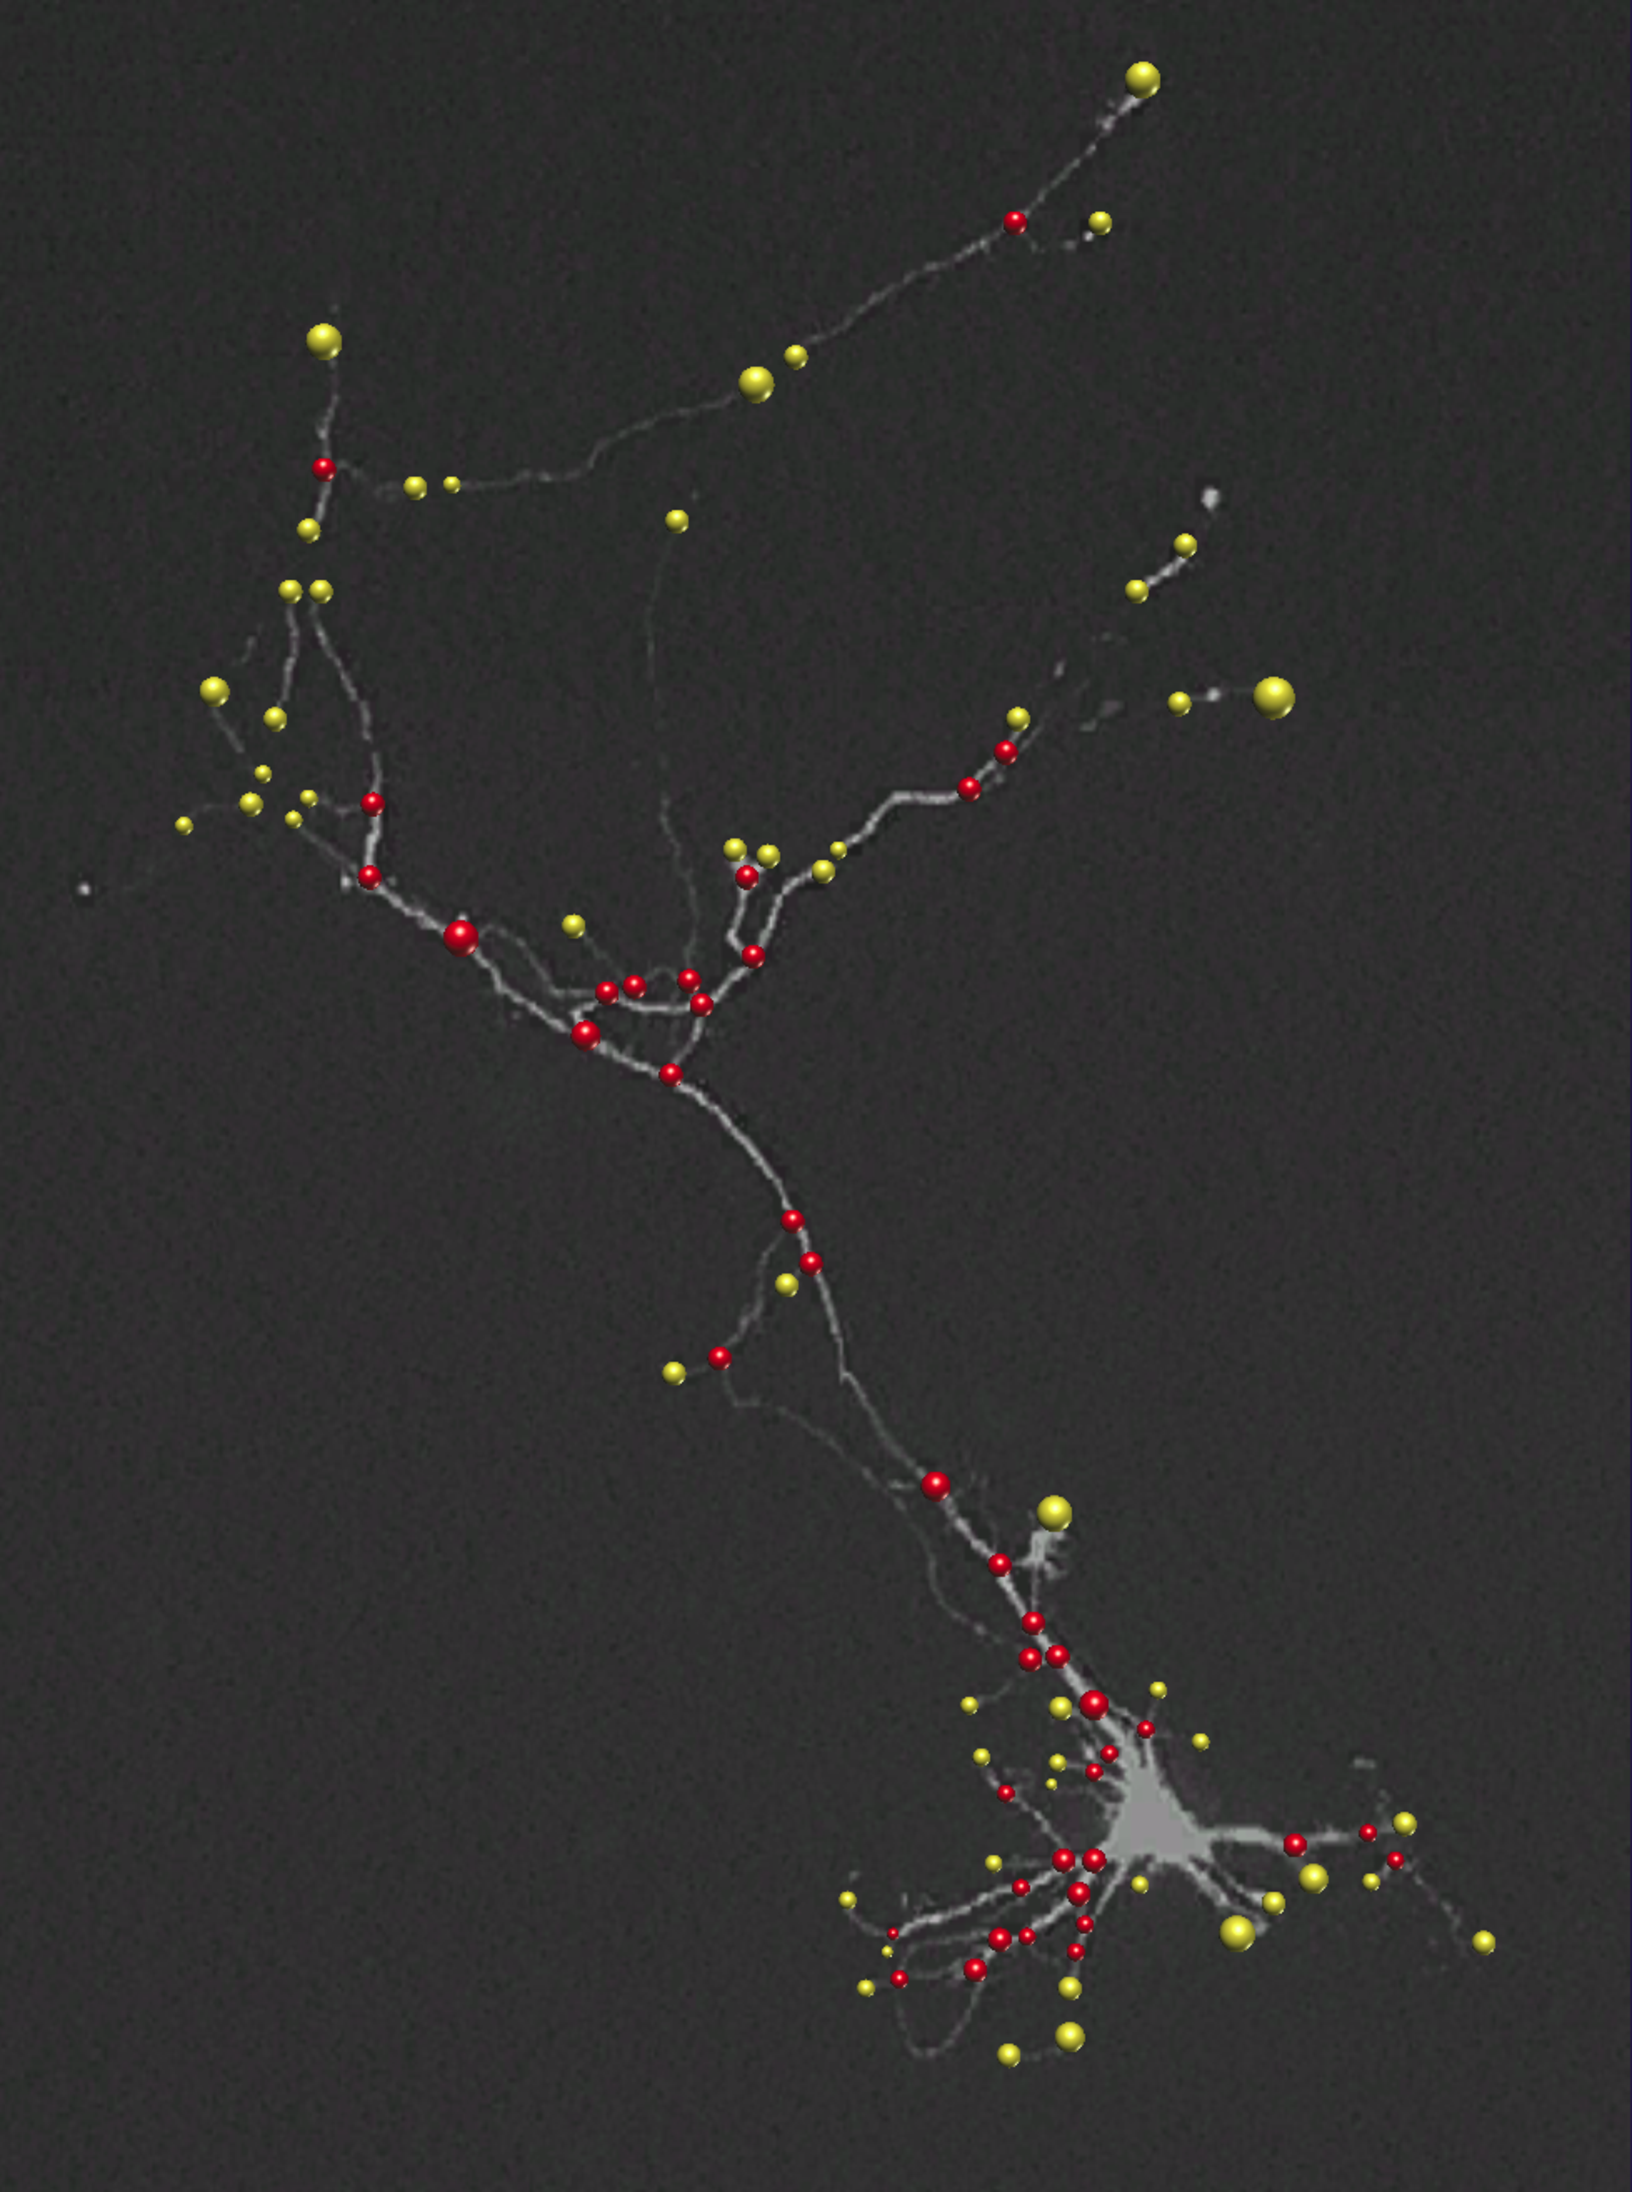
\includegraphics[width=0.5\columnwidth]{ch2_fig1}
	\caption{Fluorescence microscopy image of a neuron with manually indicated junctions (red circles) and terminations (yellow circles). The radius of each annotated critical-point region reflects the size of the underlying image structure.}
	\label{ch2_fig1_label}
\end{figure}

A key aspect of any neuron reconstruction method is the detection and localization of terminations and junctions of the dendritic (and axonal) tree, collectively called ``critical points'' in this paper (Fig.~\ref{ch2_fig1_label}), which ultimately determine the topology and faithfulness of the resulting digital representation. Roughly there are two ways to extract these critical points in neuron reconstruction \cite{al2008improved, meijering2010neuron,Basu-2013}. The most often used approach is to start with segmentation or tracing of the elongated image structures and then to infer the critical points, either afterwards or along the way, by searching for attachments and endings in the resulting subsets \cite{Dima-2002, xiong2006automated, narro2007neuronmetrics, vasilkoski2009detection, bas2011principal, chothani2011automated, Dehmelt-2011, ho2011neurphologyj, choromanska2012automatic, xiao2013app2}. This approach depends critically on the accuracy of the initial segmentation or tracing procedure, which usually is not designed to reliably capture critical points in the first place and thus often produces very fragmented results, requiring manual postprocessing to fix issues \cite{Peng-2011,Luisi-2011,Dercksen-2014}. The reverse approach is to first identify critical points in the images and then to use these as seed points for tracing the elongated image structures. Critical points can be obtained either by manual pinpointing, as in semiautomatic tracing methods \cite{meijering2004design, Schmitt-2004, narro2007neuronmetrics, lu2009semi, peng2010v3d, longair2011simple}, or by fully automatic detection using sophisticated image filtering and pattern recognition methods (discussed in the next section). The latter approach has barely been explored for neuron reconstruction, but if reliable detectors can be designed, they provide highly valuable information to the reconstruction process.

